\chapter{Quadros e registros complementares}
\label{ap:complementos}

Estes quadros detalham a comparação com a literatura, os casos, a amostra e os problemas de interface. As dimensões técnicas dos casos são práticas relatadas, não estruturas internas verificadas nas plataformas.

\begin{table}[!ht]
    \caption{Quadro comparativo dos trabalhos relacionados}
    \label{tab:relacionados}
    \centering%
    \begin{minipage}{.98\textwidth}
        \small
        \renewcommand{\arraystretch}{1.3}
        \begin{tabular*}{\textwidth}{@{}p{2.8cm}p{2.6cm}p{2.4cm}p{2.4cm}p{3.2cm}@{}}
            \toprule
            \textbf{Trabalho} & \textbf{Foco} & \textbf{Método} & \textbf{Recorte} & \textbf{Diferença metodológica e técnica}\\
            \midrule
            \citeonline{costa2022comportamento}    & Percepção do cliente    & Survey quantitativo & Brasília/DF, 2022     & Não confronta respostas com operação de casos e auditorias de interfaces\\
            \citeonline{silva2024design}            & Design e usabilidade    & Estudo exploratório  & Quixadá/CE, 2024      & Não integra requisitos dos gestores e desempenho das páginas à análise de uso\\
            \citeonline{fioreti2026aplicativos}     & Adoção + UX             & Estudo de caso e survey & Maranhão, 2026        & Usa TAM; aqui as percepções são cotejadas também com auditorias e requisitos\\
            \citeonline{schmitt2021comportamiento}  & Comportamento do consumidor & Survey correlacional & Lima/Peru, 2021       & Estuda delivery, não o cardápio no salão nem sua integração operacional\\
            \bottomrule
        \end{tabular*}
        \fonte{Elaborado pelo autor.}
    \end{minipage}
\end{table}

\begin{table}[!ht]
    \caption{Dimensões técnicas relatadas pelos gestores nos casos A a D}
    \label{tab:taxonomia-arquitetura}
    \centering%
    \begin{minipage}{.98\textwidth}
        \footnotesize
        \renewcommand{\arraystretch}{1.25}
        \begin{tabular*}{\textwidth}{>{\raggedright\arraybackslash}p{2.8cm}@{\extracolsep{\fill}}>{\raggedright\arraybackslash}p{2.0cm}>{\raggedright\arraybackslash}p{2.0cm}>{\raggedright\arraybackslash}p{2.0cm}>{\raggedright\arraybackslash}p{2.0cm}}
            \toprule
            \textbf{Dimensão} & \textbf{Caso A} & \textbf{Caso B} & \textbf{Caso C} & \textbf{Caso D} \\
            \midrule
            Dispositivo (cliente ou estabelecimento) & Tablet do estabelecimento, um por mesa & Impresso no salão; plataforma web para entrega & Celular do cliente (QR Code por mesa), além do impresso & Nenhum para o cliente; cardápio impresso \\
            Sistema próprio ou contratado & Contratado (Glow), com licença por tablet & Plataformas de entrega contratadas & Contratado como serviço (Anota AI) & Gestão contratada como serviço (Saipos) \\
            Integração com PDV, estoque e cozinha & Pedidos dos tablets e do balcão no sistema central; impressora na cozinha por rede interna; caixa central & Pedidos de telefone, WhatsApp e plataformas anotados à mão e levados à cozinha; pedido da plataforma pode ser impresso; estoque manual & Pedidos da mesa, do delivery e do iFood no sistema; caixa e estoque manuais & Pedido do garçom no sistema, com impressoras, pagamento, estoque e notas fiscais \\
            Comportamento sem internet & Segundo o supervisor, segue por rede interna depois de iniciar & Não abordado & Duas operadoras e celular como reserva & Não abordado \\
            Formato do cardápio (PDF, web, aplicativo) & Aplicativo no tablet, painel na nuvem & Impresso no salão, sem consulta ou pedido digital; web para entrega & Página web, além do impresso & Impresso; mesma arte no Instagram \\
            Identificação do cliente (cadastro, crédito) & Cartão com QR Code vinculado ao telefone & Não abordado & Nome, telefone e endereço no delivery & Nenhuma \\
            \bottomrule
        \end{tabular*}
        \fonte{Elaborado pelo autor a partir das entrevistas dos casos A a D.}
    \end{minipage}
\end{table}

\begin{table}[!ht]
    \caption{Escores dos construtos UTAUT2 e das extensões contextuais ($n = 90$)}
    \label{tab:construtos}
    \centering%
    \begin{minipage}{.98\textwidth}
        \small
        \renewcommand{\arraystretch}{1.15}
        \begin{tabular*}{\textwidth}{l@{\extracolsep{\fill}}ccccc}
            \toprule
            \textbf{Construto} & \textbf{Média} & \textbf{Mediana} & \textbf{DP} & \textbf{\% 4 ou 5} & \textbf{r entre itens} \\
            \midrule
            \inputtabela{analysis/tabelas/construtos.tex}
            \bottomrule
        \end{tabular*}
        \fonte{Elaborado pelo autor. Escala de 1 a 5; ``\% 4 ou 5'' é a proporção de escores de construto iguais ou maiores que 4. Para as extensões, que têm um item só, não há correlação entre itens.}
    \end{minipage}
\end{table}

\begin{table}[!ht]
    \caption{Perfil dos respondentes de Porto Alegre e região metropolitana ($n = 92$)}
    \label{tab:perfil}
    \centering%
    \begin{minipage}{.7\textwidth}
        \small
        \renewcommand{\arraystretch}{1.1}
        \begin{tabular*}{\textwidth}{l@{\extracolsep{\fill}}rr}
            \toprule
            & \textbf{n} & \textbf{\%} \\
            \midrule
            \inputtabela{analysis/tabelas/perfil.tex}
            \bottomrule
        \end{tabular*}
        \fonte{Elaborado pelo autor a partir das respostas ao questionário.}
    \end{minipage}
\end{table}

\begin{figure}[!ht]
    \caption{Display com QR Code em uma mesa do Ohana Açaí}
    \label{fig:ohana-qrcode}
    \centering
    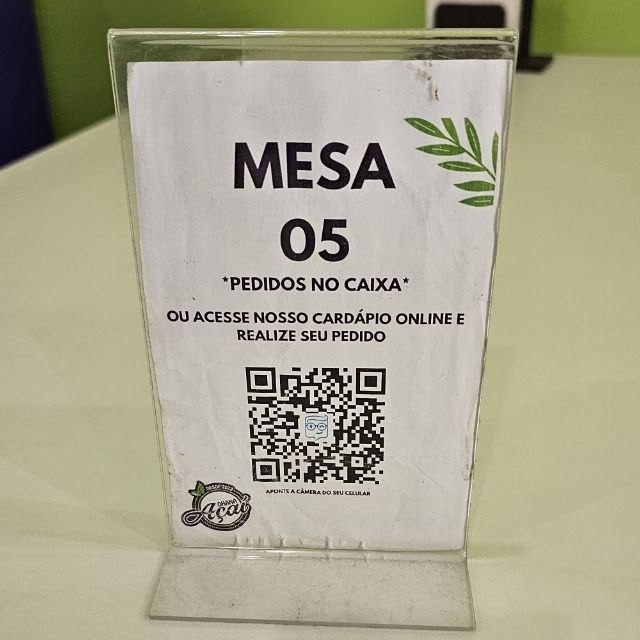
\includegraphics[width=0.5\textwidth]{images/ohana-qrcode-mesa.jpg}
    \fonte{Foto do autor, 15 nov. 2026.}
\end{figure}

\begin{table}[!ht]
    \caption{Problemas recorrentes de usabilidade e acessibilidade em cardápios digitais}
    \label{tab:problemas-ux}
    \centering%
    \begin{minipage}{.98\textwidth}
        \small
        \renewcommand{\arraystretch}{1.25}
        \begin{tabular*}{\textwidth}{>{\raggedright\arraybackslash}p{5.2cm}@{\extracolsep{\fill}}>{\raggedright\arraybackslash}p{4.6cm}>{\raggedright\arraybackslash}p{3.4cm}}
            \toprule
            \textbf{Problema relatado} & \textbf{Heurística de Nielsen} & \textbf{WCAG 2.2} \\
            \midrule
            Layout confuso ou difícil de ler & Estética e design minimalista; consistência e padrões & --- \\
            Cardápio em PDF difícil de ler no celular & Estética e design minimalista & 1.4.10 Reflow \\
            Dúvida se o pedido foi feito ou cobrado & Visibilidade do estado do sistema & --- \\
            Navegação que recarrega ou perde a posição ao voltar & Controle e liberdade do usuário & --- \\
            Necessidade de rolar a tela para comparar itens & Reconhecimento em vez de memorização & --- \\
            Interface que muda a cada atualização do sistema & Consistência e padrões & --- \\
            Item exibido, mas indisponível & Prevenção de erros; correspondência com o mundo real & --- \\
            Cadastro ou login exigido para ver o cardápio & Flexibilidade e eficiência de uso & --- \\
            Falta de ajuste de fonte e contraste & --- & 1.4.3 Contraste; 1.4.4 Redimensionar texto \\
            Zoom bloqueado pela página (auditoria) & Flexibilidade e eficiência de uso & 1.4.4 Redimensionar texto \\
            Elementos que se deslocam durante o carregamento (auditoria) & Prevenção de erros & --- \\
            \bottomrule
        \end{tabular*}
        \fonte{Elaborado pelo autor a partir das respostas ao questionário, das entrevistas, das auditorias técnicas, de \citeonline{nielsen1994heuristics} e de \citeonline{wcag22}.}
    \end{minipage}
\end{table}
